\chapter{Mathematical Models of Alzheimer's Disease}
\label{chp:2}
Mathematical modelling of AD has becoming a fertile research programme in recent
years, producing models that describe disease mechanisms and making valuable
predictions about patient trajectories \cite{raj2015network, fornari2019prion,
thompson2020, schafer2022correlating}. In particular, network models of
neurodegeneration have become increasingly popular due to the desirable balance
of complexity and explanatory power. Here, I will describe the basis for network
mathematical models of AD and some of the models used in the literature and
throughout this report.

Typically, mathematical models of neurodegeneration have focussed on modelling
the spread, accumulation and aggregation of toxic protein species, \TP and \AB.
While there have been numerous contributions focussing on continuum dynamics
\cite{weickenmeier2018multiphysics,fornari2020spatially}, as well as
probabilistic network models \cite{vogel2020spread}, I will here focus on
dynamical models on networks. More specifically, I will focus on modelling of
\TP, since it displays richer spatiotemporal dynamics that are more tightly
coupled with atrophy and symptom onset, as discussed in \cref{sec:1-bio-ad}. The
use of such network models is motivated by experimental results demonstrating
that \TP preferentially travels through axonal fibres \cite{liu2012trans,
de2012propagation, devos2018synaptic}.  
An additional benefit is that solutions to ordinary differential equations
(ODEs) on graphs are computationally less expensive to obtain than their partial
differential equation counterparts. As mentioned in
\cref{sec:1-uncertainty}, network models of AD protein pathology should aim to
describe at least transport across axons and growth via an autocatalytic process
akin to prion-like templating.

\section{Transport and the Graph Laplacian}
\label{sec:transport}
As highlighted in \cref{sec:1-uncertainty} the graph Laplacian is the central
object used to describe transport along axonal fibres. The topology of axonal
pathways can be obtained through the analysis of diffusion weighted MRI data,
such as those available from the Human Connectome Project. The output of
this analysis is a graph $G = (V, E)$, where $V$ is the enumeration of vertices
in the graph, $v_1, v_2, . . . v_n$ and $E$ the edges between them. The
transport of protein concentration between regions of the brains, vertices $V$,
can be effectively modelled using the graph Laplacian, given by:
\begin{equation}\label{eqn:laplacian_matrix}
    \mathbf{L} = \mathbf{D} - \mathbf{A},
\end{equation}
where $\tns{A}$ is an adjacency matrix encoding the connectivity between 
regions.
\begin{equation}\label{eqn:adjacency_matrix}
A_{ij} = \left\{\begin{array}{cl} 1 & \text{if an edge connects } v_i \text{ to } v_j\\ 0 
                            & \text{otherwise}\end{array}\right.,
\end{equation}
and $\tns{D}$ is the degree matrix, containing the total number of edges associated with a given vertex, 
\begin{equation}\label{eqn:degree_matrix}
D_{ij} = \delta_{ij} \sum_{j=1}^{N} A_{ij}.
\end{equation}

We can include more information about the connectivity of the brain regions by
weighting the adjacency matrix by the number and length of streamlines estimated
between regions from tractography. The choice of weighting has been extensively
discussed in \cite{putra2021braiding}. In this work, we describe transport of
toxic protein as diffusion across the brain network. The appropriate edge
weighting to describe such a process is: 
\begin{equation}
    \label{eqn:edge-weighting}
    A_{ij} = \frac{n_{ij}}{l_{ij}^{2}}
\end{equation}
where $A_{ij}$ is the edge connecting $v_i$ and $v_j$, $n_{ij}$ is the number of 
streamlines between $v_i$ and $v_j$, and $l_{ij}$ is the average length of those 
streamlines.

Using the graph Laplacian, the transport of proteins by diffusion on a graph is
given by the network heat equation: 
\begin{equation}\label{eqn:ndmodel}
    \odl{\tns{p}}{t} = -\rho \tns{L}\tns{p},
\end{equation}
where $\mathbf{p} \in \mathbb{R}^{N}$ is the protein concentration at each node
in the brain network, $\rho \in \mathbb{R}$ is the diffusion coefficient, and
$\mathbf{L} \in \mathbb{R}^{N \times N}$ is the graph Laplacian with weights
given by \cref{eqn:edge-weighting}. This model has been analysed against
data using regression studies \cite{raj2012network,raj2015network} and Bayesian
inference \cite{schafer2020network}. However, there is a wealth of evidence to
suggest that this model is not an accurate description of the prion-like process
underlying AD, since it does not account for growth coming from the prion-like
templating process \cite{jucker2013self,fornari2019prion}.

\section{Protein Proliferation}
\label{sec:growth}
\subsection{The Heterodimer Model}
To augment the network heat equation with appropriate production 
and clearance term, consider the kinetic diagram shown in \cref{fig:hxdkinetics}, 
describing Pruisner's model of prion-like propagation through templating 
\cite{prusiner1991, prusiner1998}. 
\begin{figure}[h]
    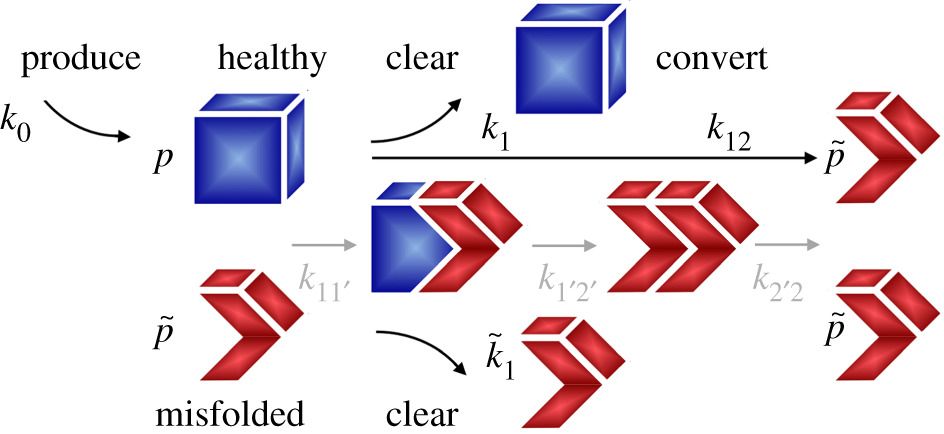
\includegraphics[width=8cm]{heterodimerkinetics.png}
    \centering
    \caption{\textbf{Reaction kinetics of the heterodimer model.} Adapted from \cite{fornari2019prion}.}
    \label{fig:hxdkinetics}
\end{figure}
There is a healthy protein concentration, $p$, and toxic protein species,
$\hat{p}$. The toxic protein binds the healthy protein with rate $k_{11'}$ and
induces a conformational change into the healthy protein, turning it into a
toxic protein at rate $k_{1'2'}$, before separating into two toxic monomers with
rate $k_{2'2}$. This is collectively summarised as rate $k_{12}$. Both healthy
and toxic protein species are cleared with a natural clearance rate of $k_1$ and
$\hat{k}_1$, respectively. With the addition of transport between regions, this
can be expressed as a pair of coupled ODEs:
\begin{subequations}
    \label{eqn:network-heterodimer}
    \begin{alignat}{3}
        \odl{p_i}{t} &=  -\rho\sum\limits_{j=1}^{N}\mathcal{L}_{ij}p_j +  k_0 &&- k_1 p_i - k_{12}p_i \hat{p}_i, 
        \label{eqn:network-heterodimer:healthy}\\
        \odl{\hat{p}_i}{t} &= -\rho\sum\limits_{j=1}^{N}\mathcal{L}_{ij}\hat{p}_j &&- \hat{k}_1 \hat{p}_i + k_{12}p_i\hat{p}_i. 
        \label{eqn:network-heterodimer:toxic}
    \end{alignat}
\end{subequations}
where $p_i \in \mathbb{R}$ and $\hat{p}_i \in \mathbb{R}$ for $i = 1 \hdots N$
are healthy and toxic protein concentration for $N$ nodes, respectively, $\rho$
is the diffusion coefficient and $\mathcal{L}_{ij}$ is the $ij$-th element of
the graph Laplacian, $\mathbf{L} \in \mathbb{R}^{N \times N}$. The combination
of Pruisner's kinetic model with the network diffusion equation provides a
mechanistic description of AD in terms of protein transport and growth
\cite{fornari2019prion}.

The physical insight obtained comes at the cost of an increased number of
parameters. For simulation purposes, this does not pose any issues, however, as
we will see in later sections, it will prove problematic for inference. Given
the temporal sparsity of data, it will be challenging to identify the parameters 
of complex models. Using a few assumptions, we can reduce the model to one 
with fewer parameters and similar global behaviour. 

\subsection{Reduction to FKPP model}
\label{sec:model-reduction-fkpp}
To simplify the heterodimer model \cref{eqn:network-heterodimer}, we can
linearise around a healthy state. First, we assume a healthy, homogenous state
with $\tilde{p}_i \ll p_i$, implying $\nicefrac{\mathrm{d}p_i}{\mathrm{d}t} = 0$ and
$-\lap{p_j} = 0$ for $i = 1 \hdots N$. Then, using 
\cref{eqn:network-heterodimer:healthy}, we can write $p$ as a function of
$\tilde{p}$
\begin{align*}
    0 &= k_0 - k_1 p_i - k_{12}p_i \hat{p}_i \\ 
    p_i(\tilde{p_i}) &= \frac{k_0}{k_1 + k_{12}\tilde{p}_i}.
\end{align*}
Linearising around $\tilde{p} = 0$, we have 
\[
    p_i(\tilde{p}_i) \approx \frac{k_0}{k_1}\left(1-\frac{k_{12}}{k_1}\tilde{p}_i\right).    
\]
Substituting this expression for $p$ into
\cref{eqn:network-heterodimer:toxic} we obtain, 

\begin{equation}\label{eqn:fkpp-goriely}
    \odl{\tilde{p}_i}{t} = - \rho \lap{\tilde{p}_j}  
                        + \beta \tilde{p} 
                         -\alpha\tilde{p}^2,
\end{equation}
where 
\begin{equation}
    \beta = \frac{k_0}{k_1}k_{12} - \tilde{k}_{1} 
    \qquad \text{and} \qquad 
    \alpha = \frac{k_0 k_{12}^2}{k_1^2}.
\end{equation}
To derive the canonical FKPP model, we make a change of variables
$\tilde{p} = c \beta\alpha^{-1}$, giving: 

\begin{equation}
    \label{eqn:fkpp-global}
    \odl{c_i}{t} = - \rho \lap{c_j} + \beta c_i \left( 1 - c_i \right)     
\end{equation}

The simulated dynamics of the FKPP model, \cref{eqn:fkpp-global}, are shown in
\cref{fig:fkpp-global}. The simulation showed has \TP seed of 50\% concentration
in the bilateral entorhinal cortex, with $\rho = 0.1$ and $\alpha = 1.2$. These
are synthetic parameters to used to illustrate the dynamics in a growth
dominated regime, $\rho \ll \alpha$. During the early stages of AD, the staging
of \TP across the connectome shares qualitative similarity with observed staging
in AD patients. However, there are some notable deficiencies that may prevent
the accurate prediction of patient disease from \TP PET observations. Notably,
the model in \cref{eqn:fkpp-global} does not account for regional variations in
tracer dynamics such as off-target binding, non-specific binding, tracer uptake
and binding-affinity. These factors are responsible for the heterogeneous SUVR
values observed in healthy individuals and and contribute to the distribution of
\TP tracer in end-stage AD subjects, as discussed in \cref{sec:1-imaging} and 
shown in \cref{fig:taustaging}. To address these issues, we next seek to
derive a model of \TP dynamics that incorporates these characteristics, whilst
still maintaining the reduced complexity that permits inference with patient
data.

\begin{figure}[H]
    \centering
    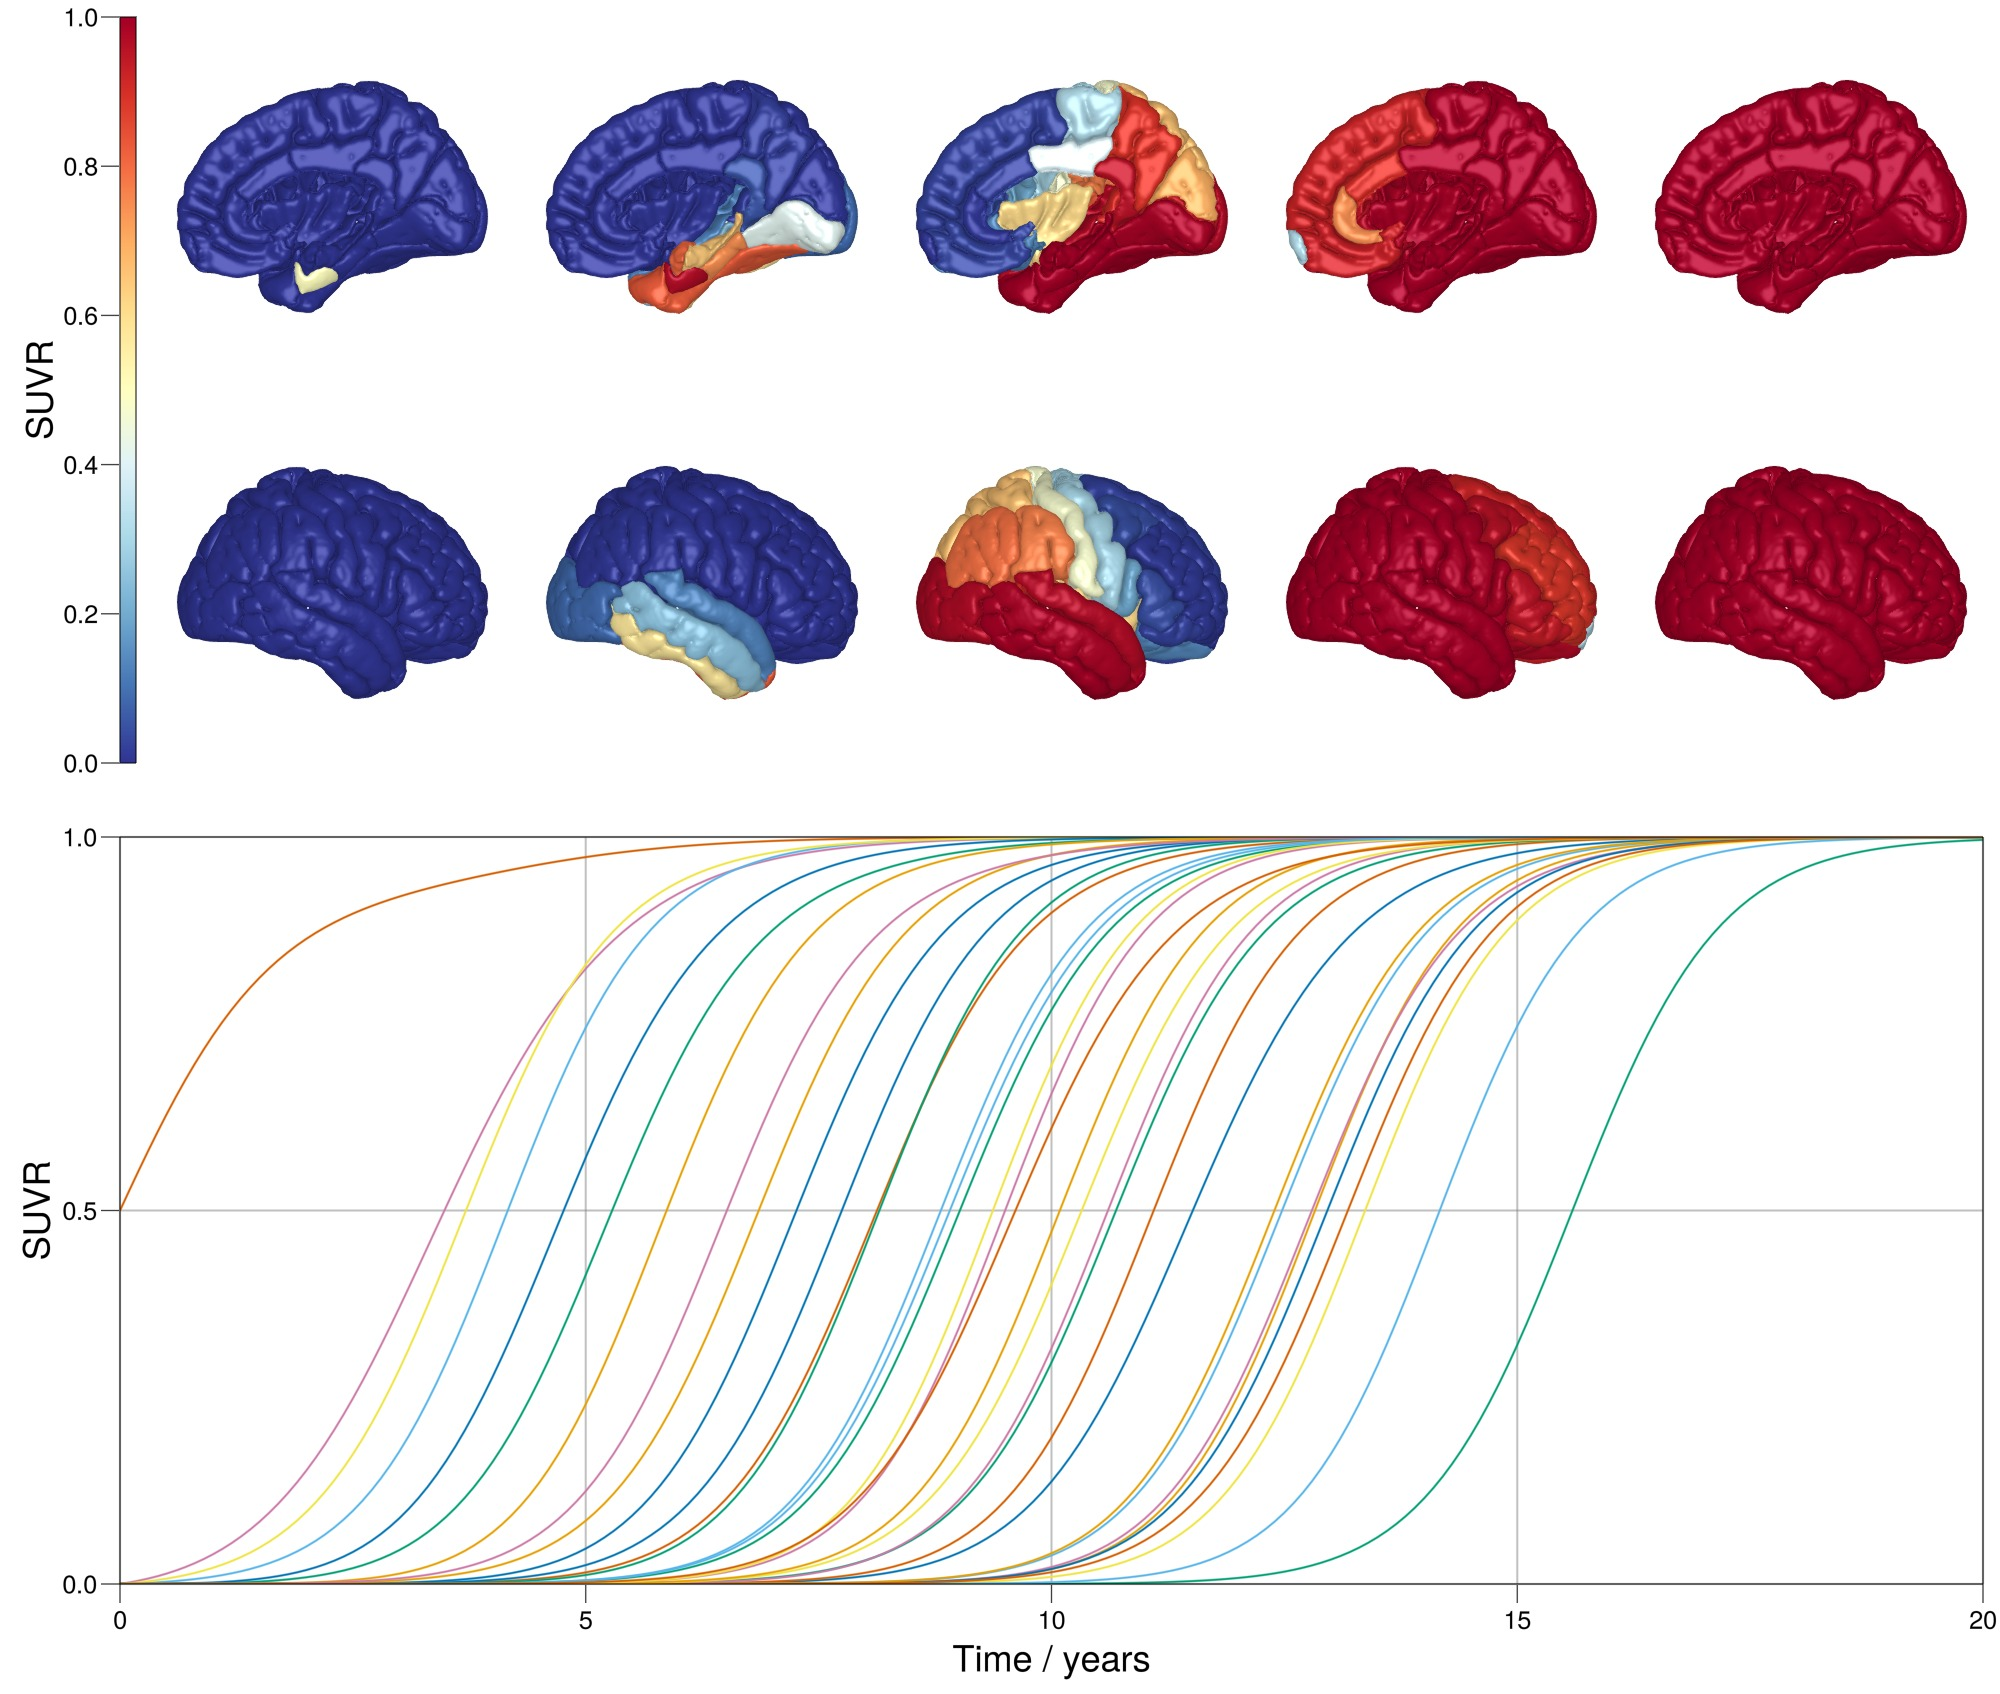
\includegraphics[width=0.9\textwidth]{local-fkpp/models/global-fkpp.jpeg}
    \caption{\textbf{Simulation from the global FKPP model}. \cref{eqn:fkpp-local}, 
    with bilateral seeding in the entorhinal cortex of 50 percent concentration, 
    $\rho = 0.1$ and $\alpha = 1.2$.}
    \label{fig:fkpp-global}
\end{figure}

\subsection{Local model of \TP pathology}
To derive a model that incorporates regional variations in tracer dynamics we
first follow the same steps to derive \cref{eqn:fkpp-goriely} from
\cref{eqn:network-heterodimer}.  We then make a change of variables to $s_i =
\tilde{p}_i + s_{0,i}$  to accommodate the potentially non-zero healthy baseline
level of observed \TP PET signal. Incorporating this change of variables, we
have: 
\begin{equation}\label{eqn:fkpp-suvr}
    \odl{s_i}{t} = - \rho \lap{\sso{j}}  
                        + \beta \sso{i} 
                         -\alpha \sso{i}^2,
\end{equation}
\[
    \beta = \frac{k_0}{k_1}k_{12} - \tilde{k}_{1} 
    \qquad
    \alpha = \frac{k_0 k_{12}^2}{k_1^2}.
\]
To determine regional carrying capacities, we again assume a healthy, homogenous
state, therefore: 
\begin{align}
    0 &= \beta \sso{i} - \alpha \sso{i}^2 \\
      &=\alpha\sso{i}\left(\beta \alpha^{-1} - \sso{i}\right).
    \label{eqn:static-fkpp}
\end{align}
Then, either $s_i = s_{0,i}$, at the minimum, or $s_i$ reaches 
its maximum when $s_i = \beta\alpha^{-1} + s_{0,i}$, which we define as
a new variable $s_{\infty,i}$, the carrying capacity. Therefore, we can rewrite
\cref{eqn:static-fkpp} as

\begin{equation}
    0 = \alpha \sso{i}\left[ \ssi{i} - \sso{i} \right].    
    \label{eqn:homogenous-local-fkpp}
\end{equation}

However, note that $s_{\infty,i} = \beta\alpha^{-1} + s_{0,i}$ implies
that the carrying capacity varies regionally only as a function of baseline
values, $s_{0,i}.$ The simplest assumption we can make to reflect regionally
varying carrying capacities, given the heterodimer model
\cref{eqn:network-heterodimer}, is to introduce a regionally varying clearance
rate of toxic protein, $\tilde{k}_1 \rightarrow \tilde{k}_{1,i}$, since it
appears only in our in carrying capacity through $\beta$ but not the uniform
growth rate $\alpha$. Therefore, the new definition for our carrying capacity is
$s_{\infty,i} = \beta_i\alpha^{-1} + s_{0,i}$ and our final model is
\begin{equation}\label{eqn:fkpp-local}
    \odl{s_i}{t} = - \rho \lap{\sso{j}}  
    + \alpha \sso{i} \left[\ssi{i} - \sso{i} \right],
\end{equation}
which defines a generative model of \TP SUVR, grounded upon a dynamical model of
\TP that accounts for regional variations in baseline values, $s_{0,i}$ and
carrying capacities $s_{\infty,i}$.


\subsection{Estimating Population Averaged Regional Parameters}
\label{sec:regionalparams}

\cref{eqn:fkpp-local} provides are a more realistic description of the 
observed \TP SUVR load in patients, however, it adds two parameter vectors, 
$\mathbf{p_0} \in \mathbb{R}^N$ and $\mathbf{p_\infty} \in \mathbb{R}^N$, for 
$N$ nodes in the brain network, therefore increasing model complexity and making 
it less practically identifiable. In this section, we provide a method
for estimating these parameters from data, allowing us to fix them ahead of
inference with individual subjects in \cref{sec:inference}. 

The approach used here extends the methods outlined in \cite{vogel2020spread}, 
in which Gaussian mixture models are used to estimate the 
probability of \TP infection. We fit a two 
component Gaussian mixture model to population level data of regional SUVR. 
For regions in which a reliable measure of \TP SUVR can be obtained, we expect 
to see two separable distributions, with one distribution capturing the 
expected, or healthy, \TP load in a given region, and one approximating the 
pathological \TP load. An example of this is given in \cref{fig:gmm-lit}, 
showing the SUVR values across the population for the inferior temporal lobe. 
In regions with a high degree of off-target binding, it is 
not possible to obtain a reliable measurement of \TP and thus making them 
difficult to model. An example of this 
can be seen in \cref{fig:gmm-lp}, showing a two component Gaussian 
mixture model fitted to the left putamen, a region known to display a high 
degree of off-target binding \cite{choi2018off}. These features associated wtih 
off-target binding are present throughout the subcortex, with exceptions in the 
hippocampi and amagydalae \cite{choi2018off, vogel2020spread}. To prevent
contamination with modelling results, we exclude these regions from our
connectome based models.

Using the remaining regions, $N = 72$, we estimate \p0 as the mean of 
the distributions describing describing healthy uptake. To approximate the 
carrying capacity, \pI, we use the 99-th percentile of the 
distributions describing pathological \TP burden. The derived baseline 
values and carrying capacities are visualised on the cortex in 
\cref{fig:baseline-capacities,fig:carrying-capacities}, respectively.
The cortex wide characteristics in baseline values, \p0 and carrying capacities,
\pI, are summarised in \cref{table:regionalparams}. The values of \p0 have
no important distinguishing features, with low variance around the mean. As
expected, the values of \pI are all higher than those of \p0. Additionally,
there is substantially more spread in the values of \pI across brain regions,
showing that carrying capacities are not uniform but rather have important
variations. These differences are more readily discerned from
\cref{fig:carrying-capacities}, in which it can be seen that the temporal,
occipital and lateral frontal regions have particularly high SUVR ranges. As
expected, the carrying capacities are consistent with in-vivo \TP staging and
longitudinal \TP PET neuroimaging studies (see \cref{fig:taustaging}) 
\cite{SCHOLL2016971,lowe2016, cho2016vivo}.

\begin{table}[h]
        \centering
        \begin{tabular}{lrrrr}
          \hline\textbf{Parameter} & \textbf{mean} & \textbf{std} & \textbf{min} & \textbf{max} \\\hline
          \p0 & 1.1108 & 0.0609 & 0.9818 & 1.2384 \\
          \pI & 2.4177 & 0.3773 & 1.9027 & 3.3321 \\\hline
        \end{tabular}
        \caption{Table of fixed parameters}
        \label{table:regionalparams}
\end{table}

\begin{figure}[H]
    \centering
    \begin{subfigure}{0.45\textwidth}
        \centering
        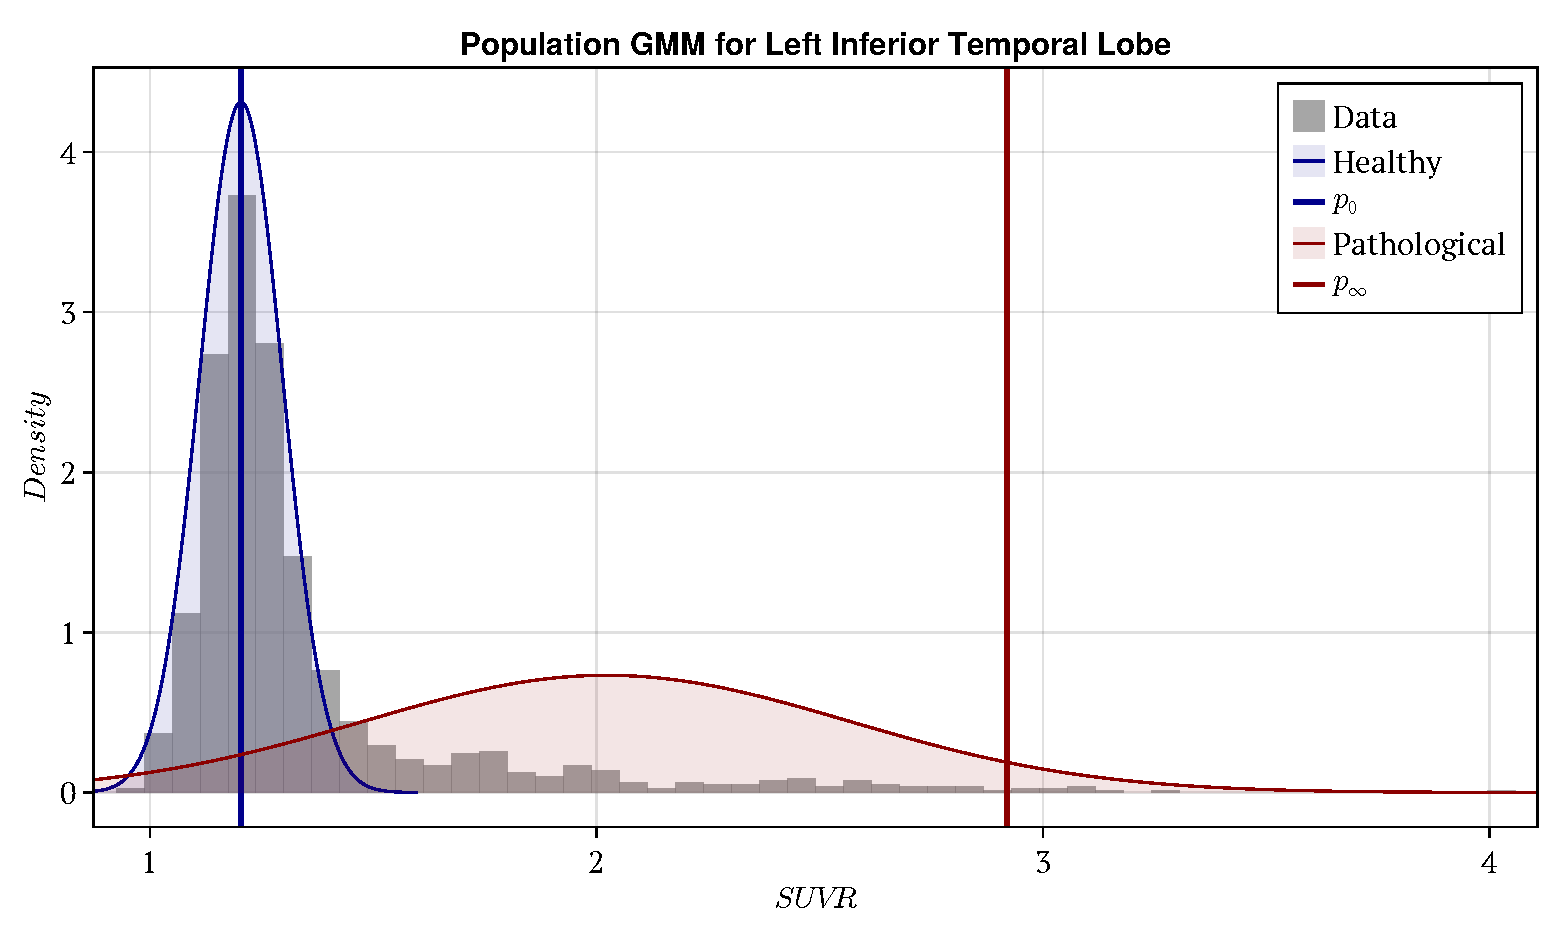
\includegraphics[width=\textwidth]{local-fkpp/models/gmm-lIT.pdf}
        \caption{GMM inferior temporal}
        \label{fig:gmm-lit}
    \end{subfigure}
    \begin{subfigure}{0.45\textwidth}
        \centering
        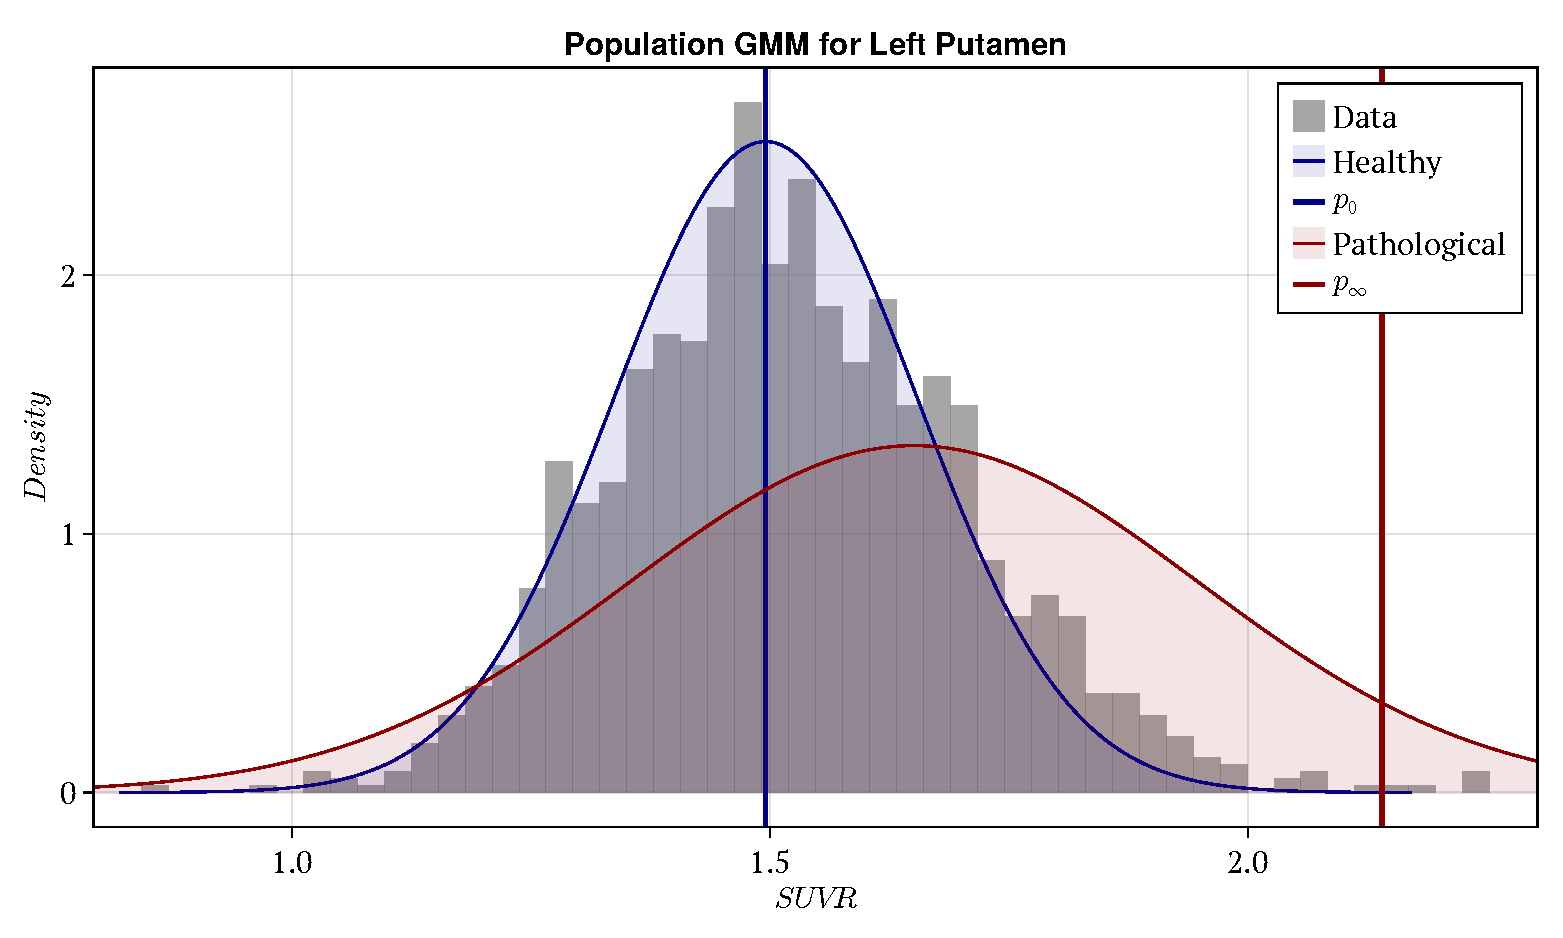
\includegraphics[width=\textwidth]{local-fkpp/models/gmm-lPutamen.pdf}
        \caption{GMM putamen}
        \label{fig:gmm-lp}
    \end{subfigure}
    
    \begin{subfigure}{0.95\textwidth}
        \centering
        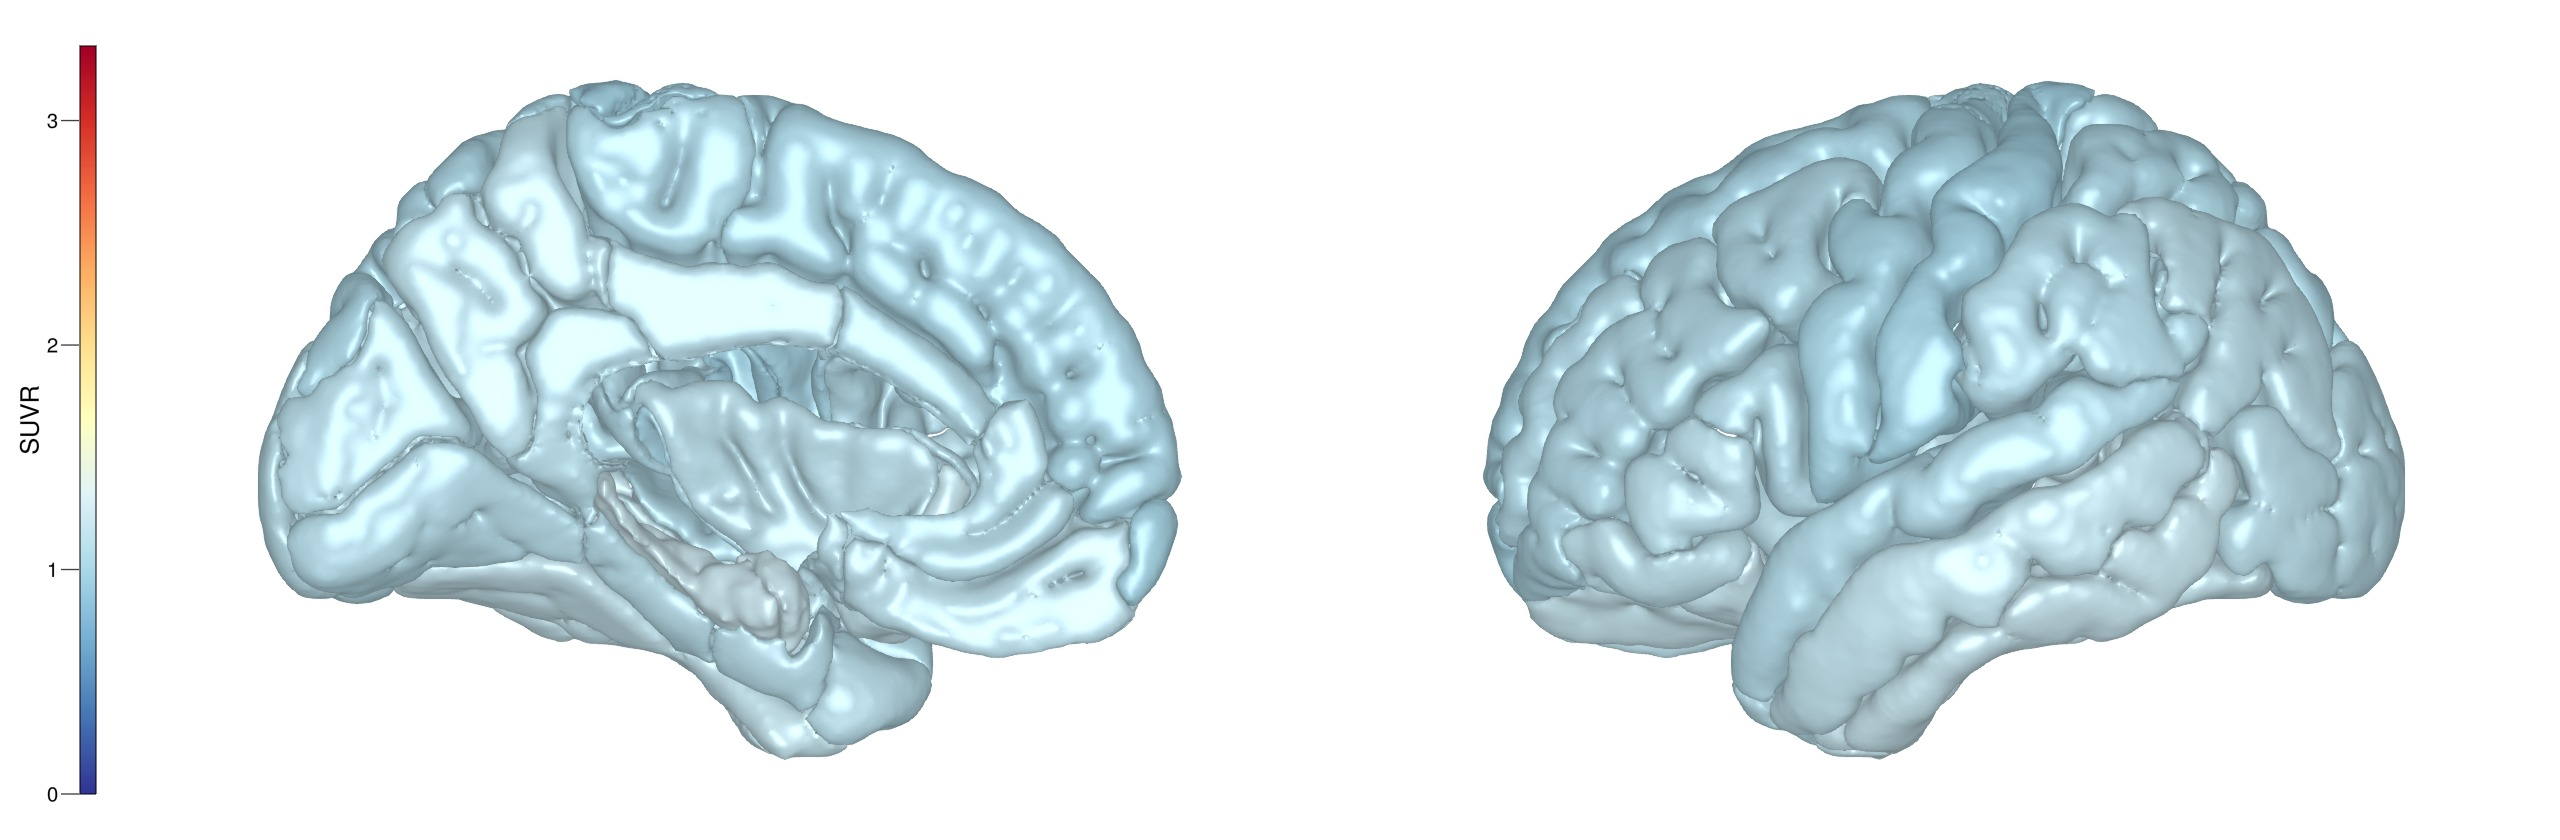
\includegraphics[width=\textwidth]{local-fkpp/models/baseline-capacities.jpeg}
        \caption{Baseline values}
        \label{fig:baseline-capacities}
    \end{subfigure}
    
    \begin{subfigure}{0.95\textwidth}
        \centering
        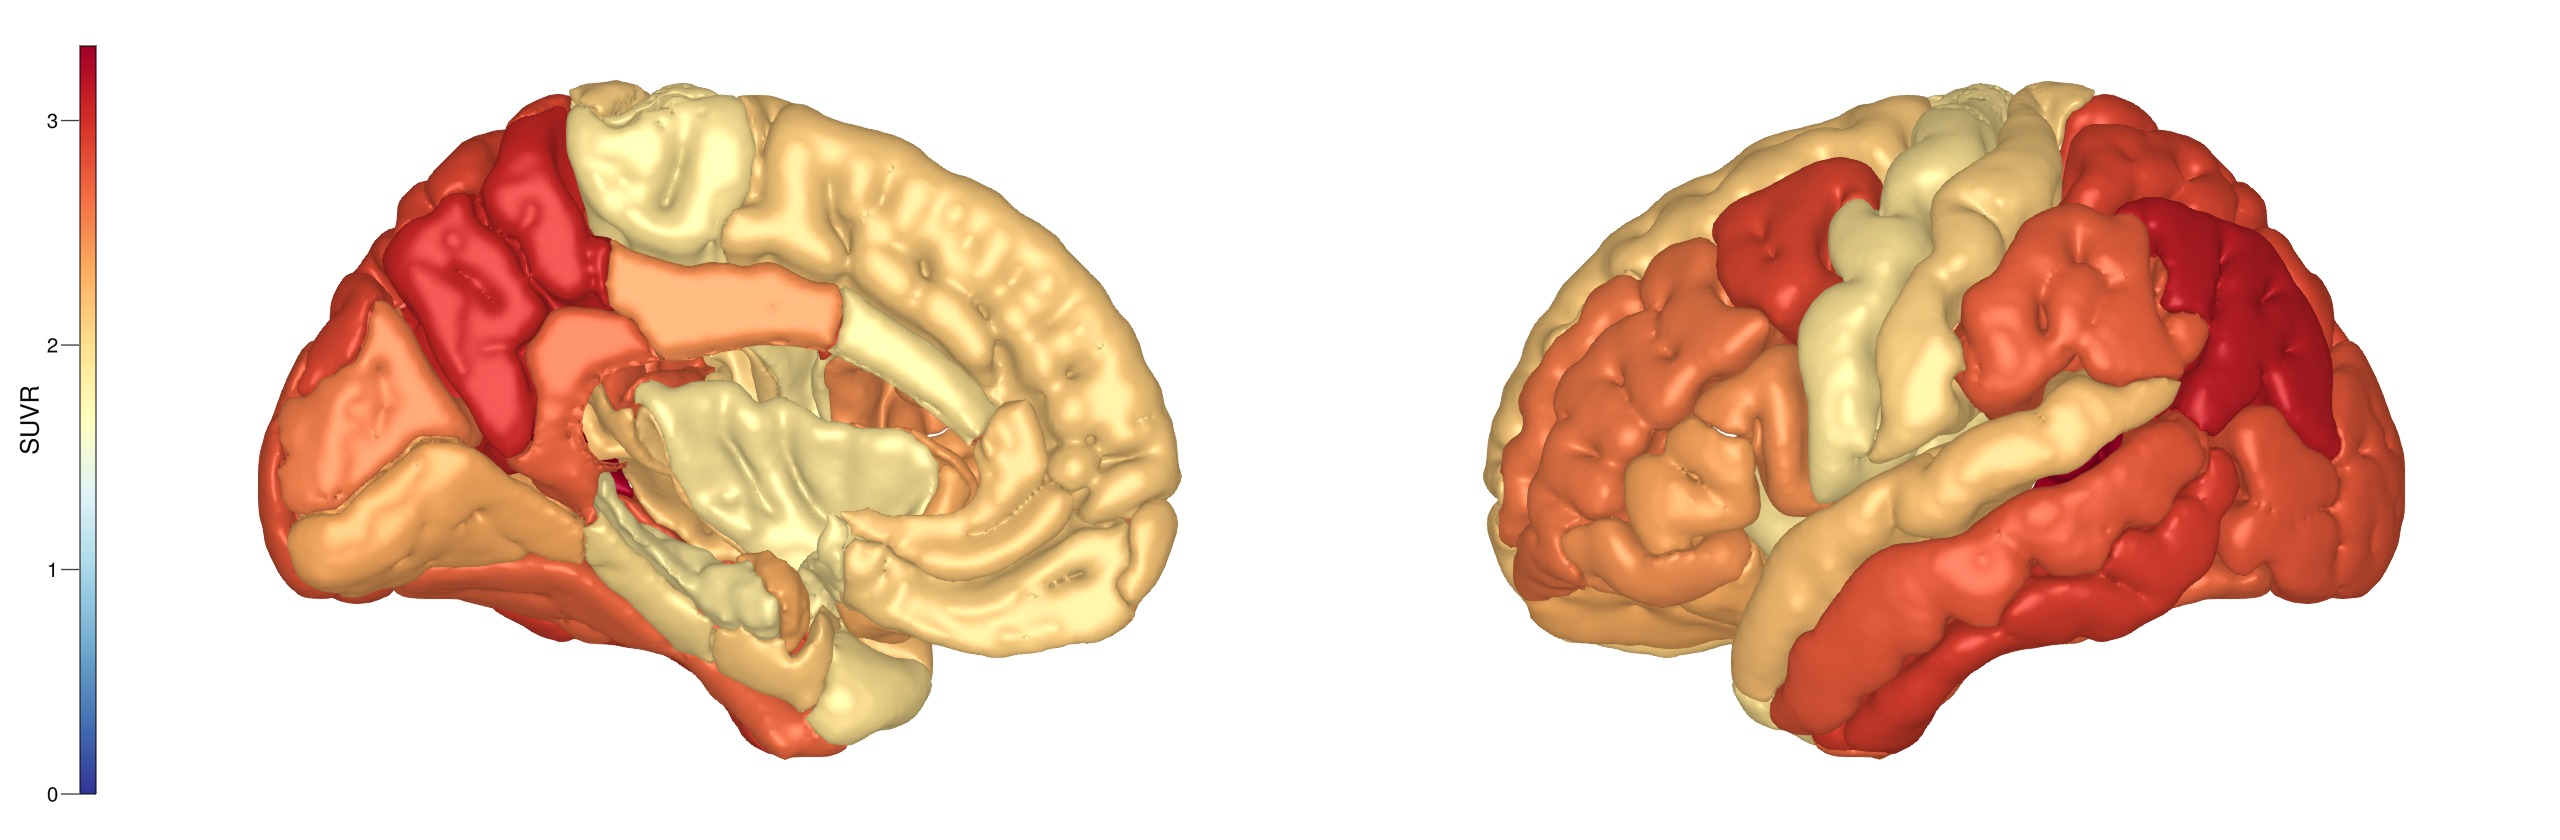
\includegraphics[width=\textwidth]{local-fkpp/models/carrying-capacities.jpeg}
        \caption{Carrying capacity values}
        \label{fig:carrying-capacities}
    \end{subfigure}

    \caption{\textbf{Population level Gaussian mixture modelling}.
    \cref{fig:gmm-lit,fig:gmm-lp} show a two component Gaussian mixture
    model fit to population level SUVR data from the left inferior temporal lobe
    and left putamen, respectively. \cref{fig:baseline-capacities} shows the mean
    of the \TP- negative distribution, $\mathbf{p}_{0}$, on the left hemisphere. 
    \cref{fig:carrying-capacities} shows the 99th percentile of the \TP+ 
    distribution, $\mathbf{p}_\infty$, on the left hemisphere}
    \label{fig:gmm}.
\end{figure}

The simulated dynamics of the local FKPP model, \cref{eqn:fkpp-local}, using the
approximated values of $\mathbf{p}_{0}$ and $\mathbf{p}_\infty$ can be seen in
\cref{fig:fkpp-local}. As with \cref{fig:fkpp-global}, we use synthetic
parameters to illustrate dynamics in a growth dominated regime. The staging
bears close resemblance to Braak staging, namely that with seeding in the
bilateral entorhinal cortex is followed by invasion of the temporal cortices,
followed occipital and frontal regions \cite{cho2016vivo, SCHOLL2016971},
whereas the staging obtained from \cref{eqn:fkpp-global} fails to capture
preferred invasion of frontal regions relative to pre/post central gyrus. The
main difference between the models comes from local variations in growth. In the
time series shown in \cref{fig:fkpp-global}, the concentration at all nodes grow
at the same rate, however, due to the local differences in baseline values and
carrying capacities in the local FKPP model, the concentration at each region
grow at different rates (proportional to the regional carrying capacities),
which can be seen in the time series of \cref{fig:fkpp-local}. As a result, the
model is more representative of observed PET data and the Braak staging we
expect to see in \TP SUVR.

\begin{figure}[H]
    \centering
    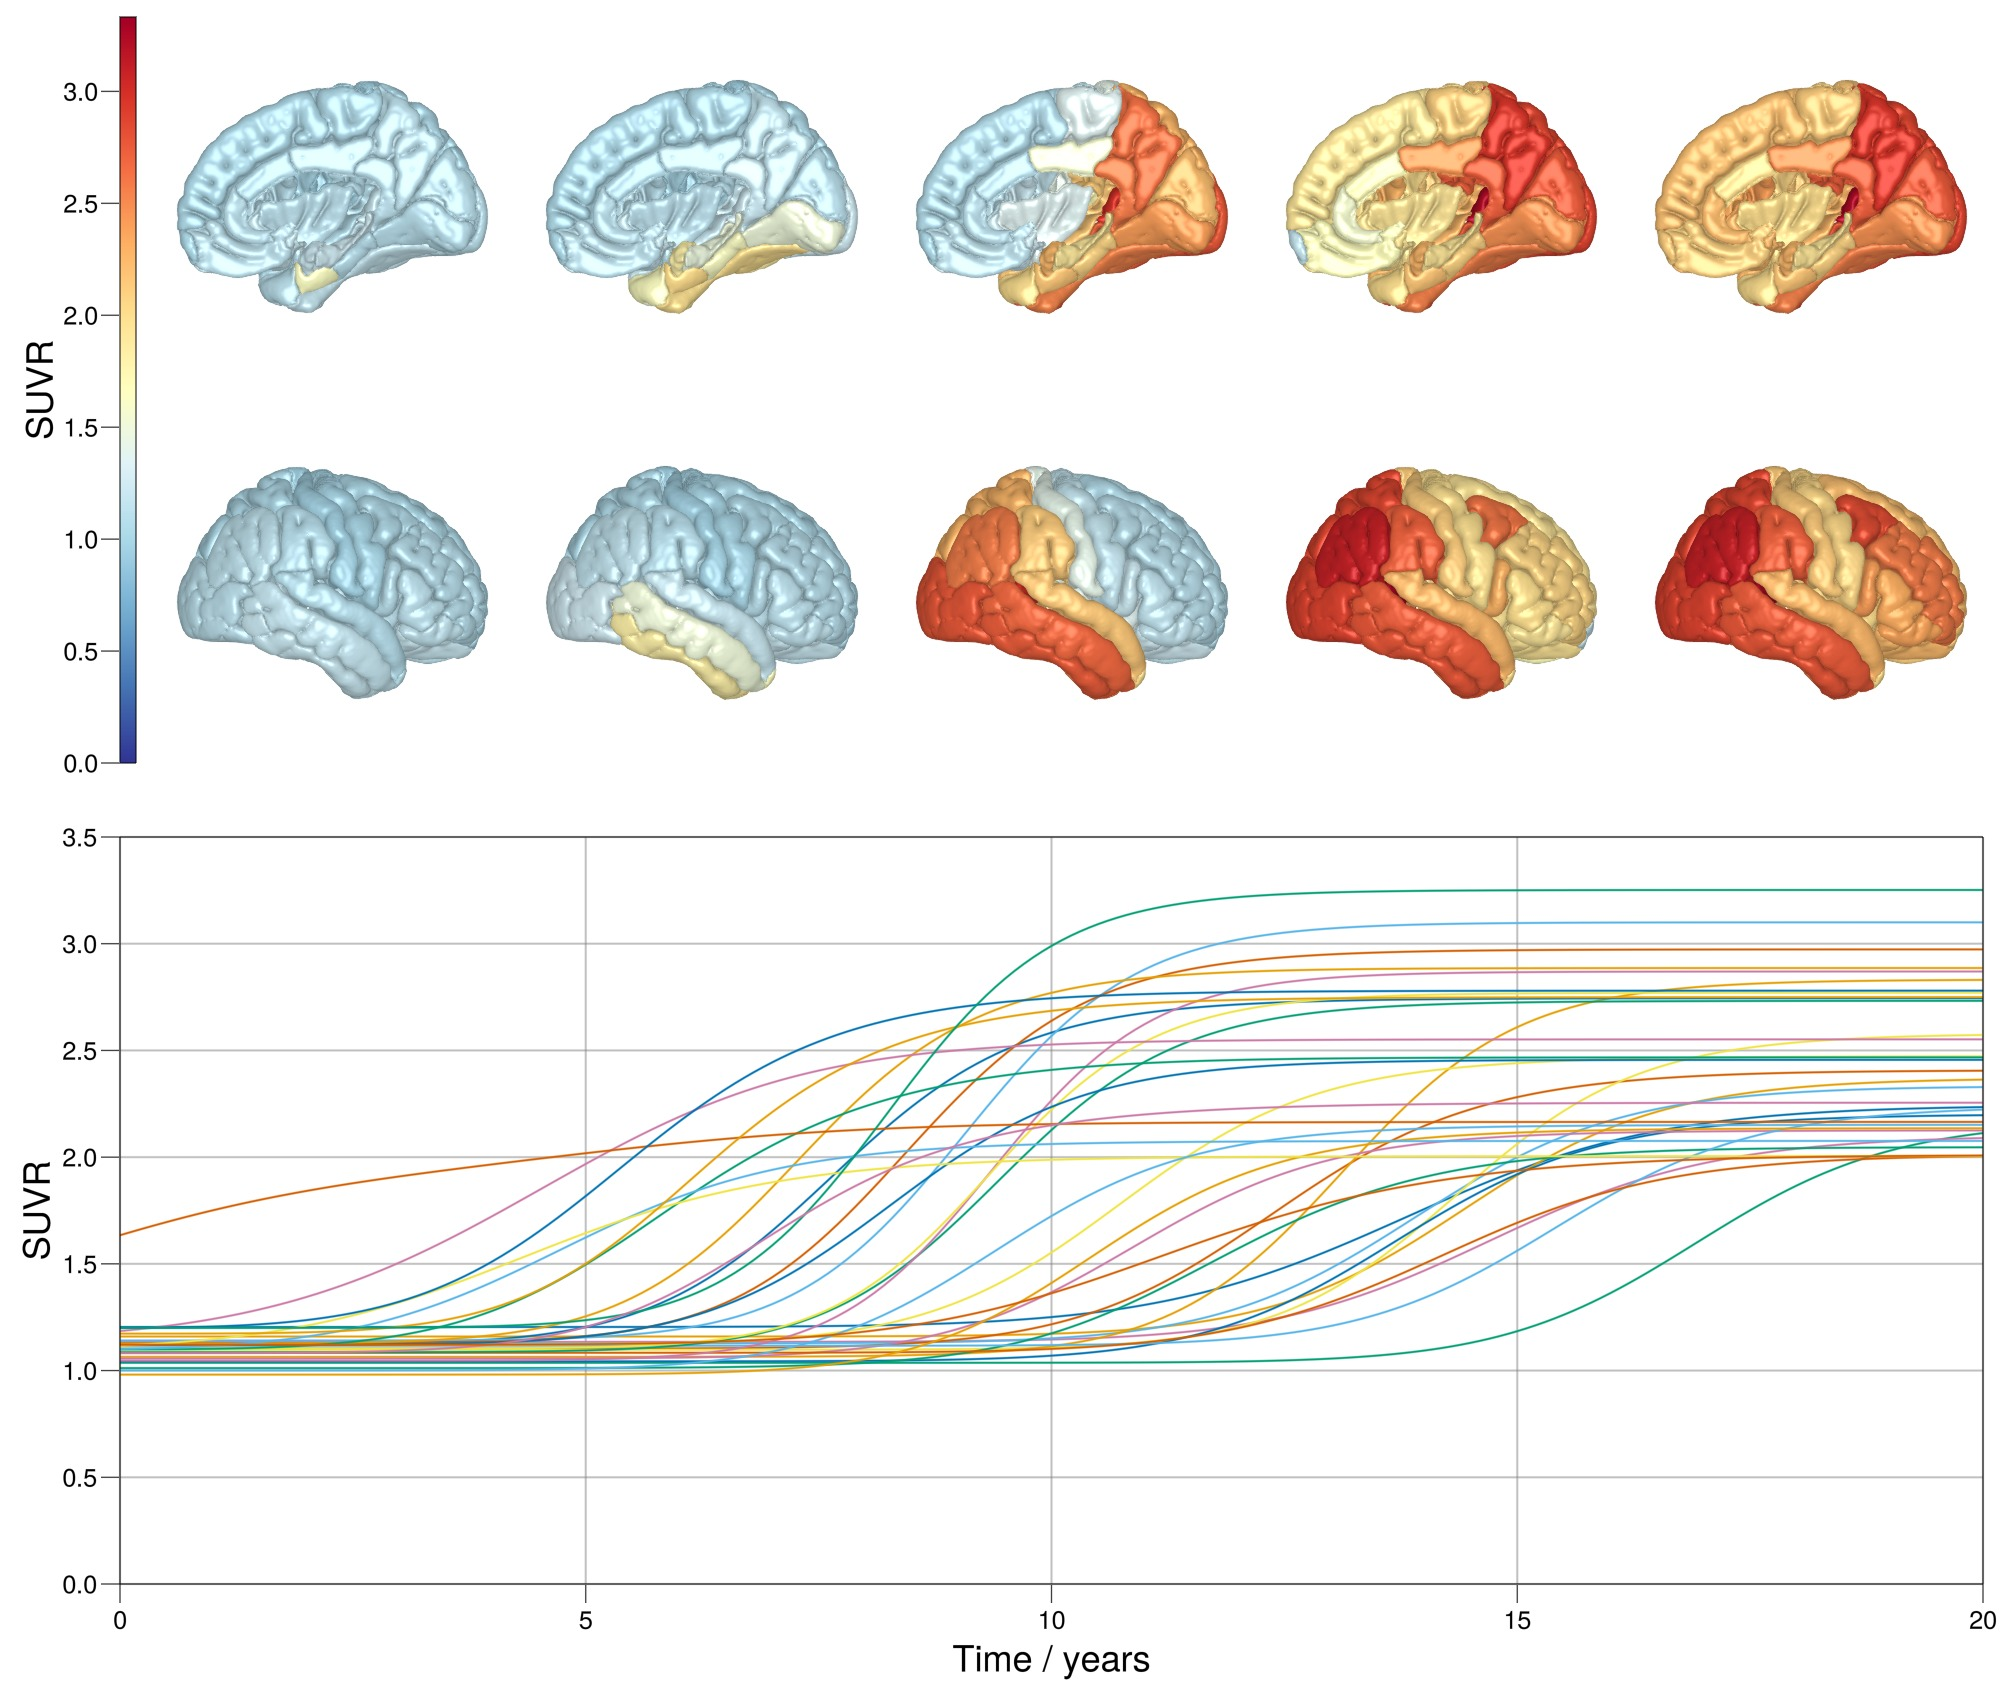
\includegraphics[width=0.9\textwidth]{local-fkpp/models/local-fkpp.jpeg}
    \caption{\textbf{Simulation from the local FKPP model} \cref{eqn:fkpp-local}, 
    with bilateral seeding of 50 percent in the entorhinal cortex, $\rho = 0.2$
    and $\alpha = 1.75$. The seeding concentration is taken as the mean of $p_0$
    and $p_\infty$ for the entorhinal cortex.}
    \label{fig:fkpp-local}
\end{figure}


\section{Identifying Uncertainty}
\label{sec:inference-example}
So far, we have discussed how different models may account for AD. In practice,
one would want to use the models for prediction. In this case, the model
requires calibration to find the most likely parameter values. In a system of
ODEs, the trajectory is uniquely determined by the initial conditions and the
parameters. The process of solving this trajectory is the forward problem. The
inverse problem, which is of concern to us for inference, asks whether the
initial conditions and parameters can be determined from partially observed
trajectories. While traditional frequentist methods have been used in the
literature \cite{raj2015network,vogel2020spread}, here, we will explore Bayesian
inference since it offers a more complete account of uncertainty.

\subsection{Probabilistic Models and Bayesian Inference}

Consider the following data generating process:
\begin{equation}\label{eqn:general-forward-model}
    \tns{x} =  \tns{g}(\tns{u}_0,  \mathbf{t}; \boldsymbol{\theta}, \tns{L}) + \boldsymbol{\epsilon}, 
\end{equation}
where $\tns{x}$ is vector of data that is assumed to be generated by integrating
a function of the form in \cref{equ:general-system}, with initial conditions
$\mathbf{u}_0$ and model parameters, $\boldsymbol{\theta}$, plus measurement
error. Using inference, we hope to identify distributions for unobserved parts
of the system, i.e. model parameters and measurement error. We do this using
Bayesian inference, where the problem corresponds to learning a posterior
density  
$p(\boldsymbol\theta \mid \mathbf{x})$ from a joint probability distribution of
the model and data $p(\boldsymbol\theta , \mathbf{x})$. This is achieved by
making use of the Bayes' theorem.
\begin{equation}\label{eqn:bayesrule}
    \underbrace{p(\boldsymbol{\theta} \mid \mathbf{x})}_{posterior} = 
    \frac{\overbrace{p(\mathbf{x} \mid \boldsymbol{\theta})}^{likelihood}
    \overbrace{p(\boldsymbol{\theta})}^{prior}}
    {\underbrace{p(\mathbf{x})}_{evidence}},
\end{equation}
where $\boldsymbol{\theta}$ is the set of unknown model parameters and $\tns{x}$
are the observations. For even mildly high-dimensional problems, solving for
$p(\boldsymbol\theta, \mid \tns{x})$ becomes intractable using analytic
techniques, since it relies on performing integration over increasingly large
domains to evaluate the evidence term. The evidence term can be reformulated as: 
\begin{equation}
    {p(\mathbf{x})} = \int p(\mathbf{x} , \mathbf{\boldsymbol{\theta}}) \mathrm{d}\mathbf{\boldsymbol{\theta}},
\end{equation}
which shows explicitly that it is necessary to integrate over all of the
dimensions of $\boldsymbol{\theta}$ to compute $p(\tns{x})$. Markov chain Monte
Carlo (MCMC) methods are a popular class of algorithms used for sampling from
the unnormalised posterior distribution, the most common among them being the
Metroplis-Hastings (MH) algorithm. In this work, we use Hamiltonian Monte Carlo
(HMC), an MCMC method that is particularly useful for fast and accurate
inference of high dimensional models with covarying parameters. In general, 
MCMC methods work by sampling from the unnormalised posterior,
denoted $\pi(\boldsymbol\theta)$, which is proportional to the full posterior: 
\begin{equation}
    \label{eqn:unnormalisedpdf}
    \pi(\boldsymbol\theta) = p(\mathbf{x} \mid \boldsymbol{\theta})p(\boldsymbol{\theta}) \propto 
    \frac{p(\mathbf{x} \mid \boldsymbol{\theta})p(\boldsymbol{\theta})}{p(\mathbf{x})}
\end{equation}
To draw samples that capture the posterior, we construct a Markov
process with a transition function $Q(\boldsymbol\theta' \mid
\boldsymbol\theta^t)$, where $\boldsymbol\theta$ is the accepted parameters at
time $t$, and $\boldsymbol\theta'$ are the proposed parameters for $t+1$. Given
certain conditions, this transition function defines a Markov process whose
stationary distribution equals the unnormalised posterior. In random walk MH,
$Q(\boldsymbol\theta' \mid \boldsymbol\theta^t)$ is chosen to be a diagonal
multivariate Normal distribution centred around $\boldsymbol\theta^t$,
$\mathcal{N}(\boldsymbol\theta^t, \boldsymbol\Sigma)$. Proposals
parameters are accepted based on the following if 
\begin{equation}
    u \leq \min\left(1, 
    \frac{\pi(\boldsymbol\theta') Q(\boldsymbol\theta' \mid \boldsymbol\theta^t)}
    {\pi(\boldsymbol\theta) Q(\boldsymbol\theta^t \mid \boldsymbol\theta')}\right)       
\end{equation}
where $u$ is sampled from a uniform distribution, $u \sim \mathcal{U}(0, 1)$,
and rejected otherwise. This Markov process asymptotically converges to the true
posterior distribution as the number of samples tends to infinity. The
transition function used in random walk MH imbues some notable deficiencies that
limit their utility in tackling high dimensional problems. In high dimensional
spaces, the probability that random proposals will be accepted decreases
substantially and therefore the sampler can not efficiently explore posterior
space. This can lead to unfeasibly slow convergence times. HMC obviates this
problem by using a more sophisticated transition function to make proposals. In
HCM the posterior is represented as a Hamiltonian function and proposals are
generated by simulating the dynamics associated with the Hamiltonian. By doing
so the transition function utilises the geometry of posterior space and the
gradients therein to generate samples that have a high probability of being
accepted \cite{betancourt2017conceptual, neal2011mcmc}. This is true even in
high dimensional spaces with highly covarying parameters, making it an attractive
alternative to MH. In the following work we a No-U-Turn-Sampler (NUTS), a HMC
sampler which adaptively finds the optimal step size with which to simulate the
Hamiltonian \cite{hoffman2014no}.

\subsection{An Example Problem}
An example of the probabilistic modelling process is shown in
\cref{fig:fkpp-bayes}. In this example, synthetic data has been generated from
an FKPP model \cref{eqn:fkpp-global}, with an initial protein
concentration seeded in the entorhinal cortex, $\mathbf{u}_0$, shown in
(\cref{fig:fkpp-data}). In this case, the synthetic data has no added noise,
allowing us to test that that the model is identifiable under ideal conditions.
Next, assuming data $\mathbf{x}$ in \cref{eqn:general-forward-model} have
independent and identical Gaussian noise, $\boldsymbol{\epsilon} \sim
\mathcal{N}(0, \sigma^2\mathbf{I})$, our likelihood is given by: 
\[
    p(\mathbf{x} \mid \boldsymbol{\theta}, \sigma, \mathbf{u}_0, \mathbf{t}) = \mathcal{N}(\mathbf{g}(\mathbf{u}_0, \mathbf{t}, \boldsymbol{\theta}, \mathbf{L}), \sigma^2\mathbf{I}).
\]
We can now define priors on the FKPP model parameters, $\theta = \{\rho,
\alpha\}$, and noise parameter, $\sigma$ to define a posterior,
\[
    p(\boldsymbol{\theta}, \sigma \mid \mathbf{x}, \mathbf{u}_0, \mathbf{t}) = p(\mathbf{x} \mid \boldsymbol{\theta}, \sigma, \mathbf{u}_0, \mathbf{t})\,p(\boldsymbol{\theta}, \sigma),
\]
and begin to make use of sampling methods. The prior model encapsulates our
initial beliefs about the data and should generate synthetic data that covers
the observed data. This is seen in \cref{fig:fkpp-prior}, with a truncated
standard normal distribution for $\rho$ and a standard normal prior for
$\alpha$. Trajectories of the FKPP model from the prior are shown in grey and
sufficiently cover the data points, here shown only for the left hippocampus.
With the data and model in place, we use NUTS to sample from the posterior. The
posterior densities can be seen in \cref{fig:fkpp-posterior}. The true values of
the parameters are recovered with very little variation and the posterior
trajectories perfectly capture the observations, indicating that the FKPP model
is identifiable in this idealised case.

\begin{figure}[h]
    \centering
    \begin{subfigure}[b]{0.8\textwidth}
        \centering
        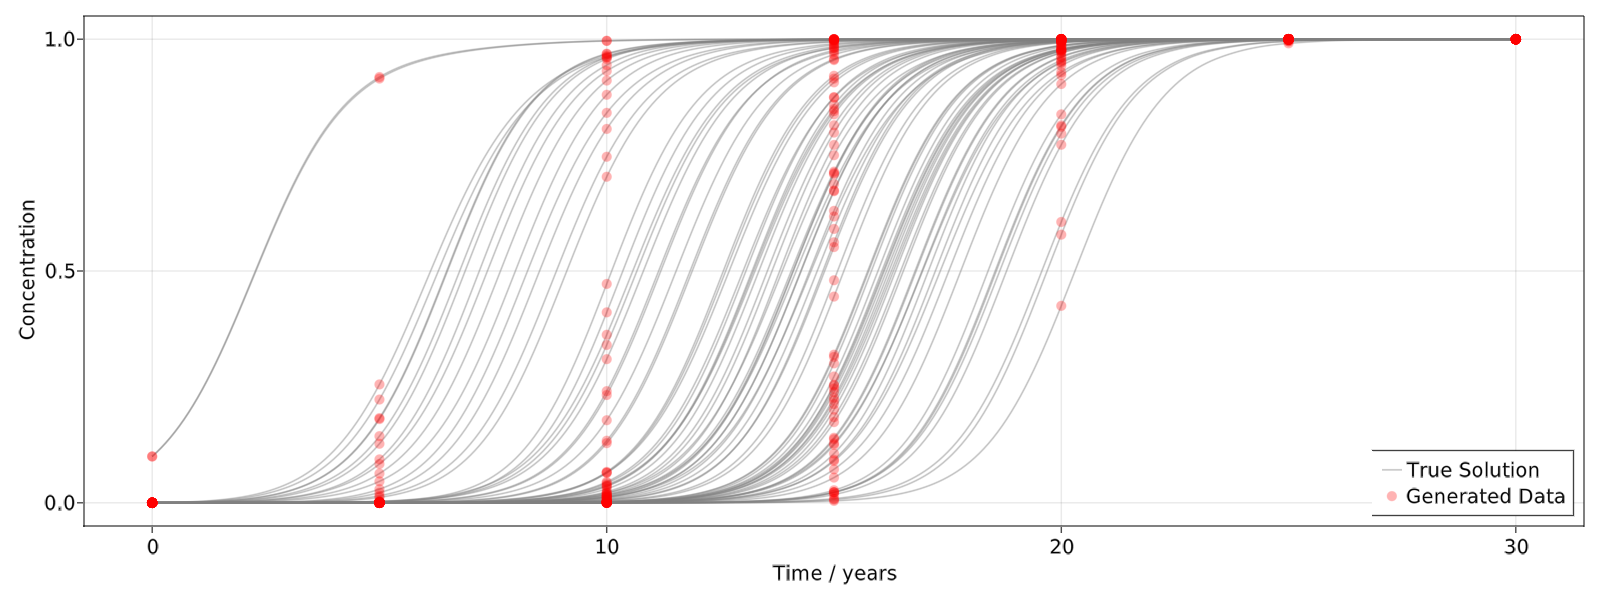
\includegraphics[width=\textwidth]{fkpp/data.png}
        \caption{FKPP solution and synthetic data}
        \label{fig:fkpp-data}
    \end{subfigure}
    \begin{subfigure}[b]{0.8\textwidth}
        \centering
        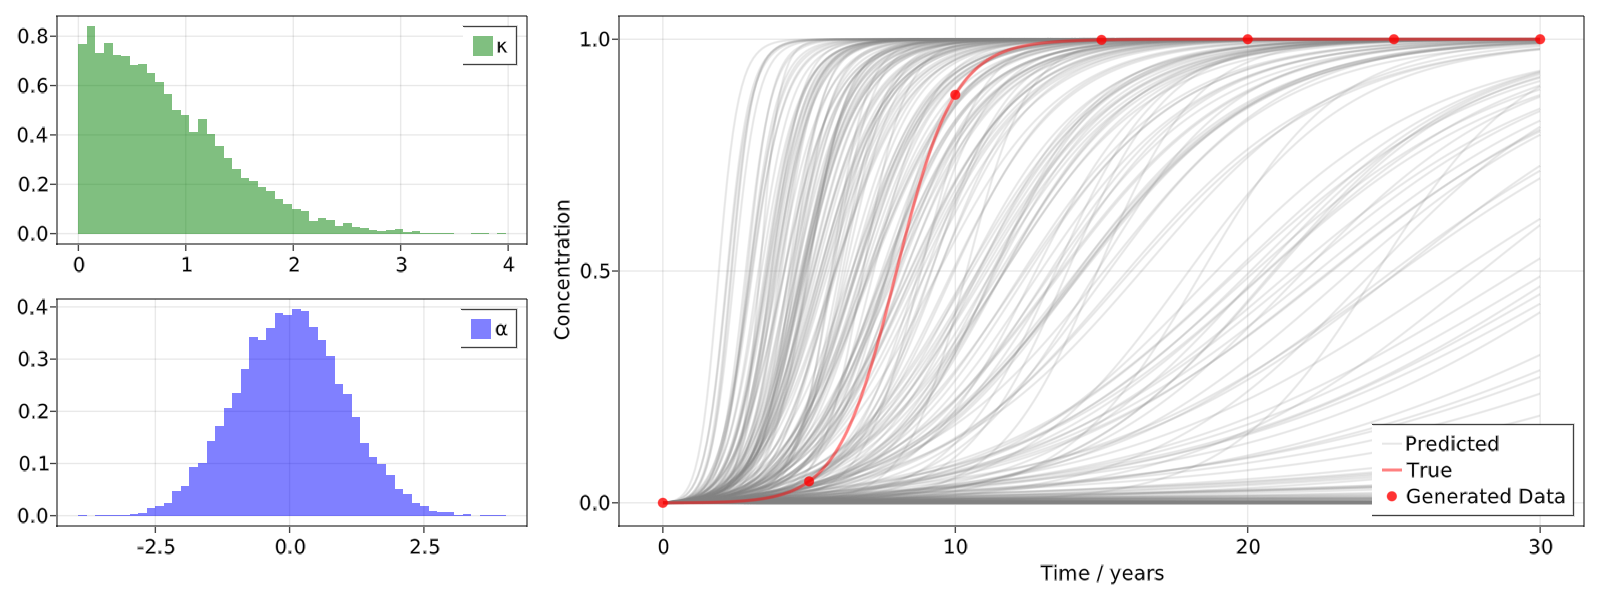
\includegraphics[width=\textwidth]{fkpp/prior_predictive.png}
        \caption{Prior distribution with sample trajectories}
        \label{fig:fkpp-prior}
    \end{subfigure}
    \begin{subfigure}[b]{0.8\textwidth}
        \centering
        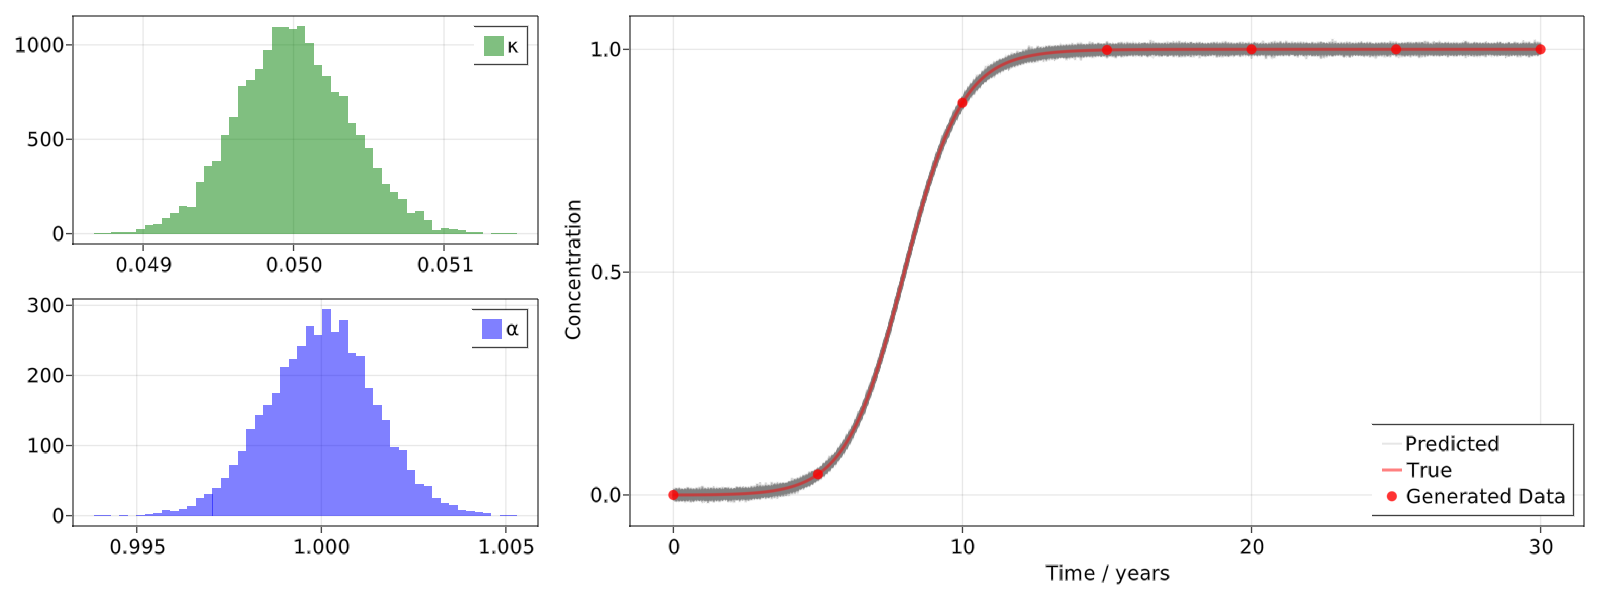
\includegraphics[width=\textwidth]{fkpp/posterior_predictive.png}
        \caption{Posterior distributions with sample trajectories}
        \label{fig:fkpp-posterior}
    \end{subfigure}    

    \caption{\textbf{Probabilistic modelling framework}. \textbf{(a)} Solution to the FKPP model (grey) with initial 
    seeding concentration of 0.1 in the entorhinal cortex, $\rho = 0.05$ and $\alpha = 1.0$, and 
    synthetic data (red) generated by taking solution values at every 5 years. \textbf{(b)} Left: Prior distribution for 
    parameters: $\rho \sim \mathcal{N}^+(0, 1)$, $\alpha \sim \mathcal{N}(0,1)$. Right: FKPP 
    solution trajectories for the right hippocampus using parameters drawn from the prior distributions.
    \textbf{(c)} Left: Posterior distributions obtained using NUTS. Right: FKPP solutions for the right hippocampus 
    using parameters drawn from the posterior distributions.}
        \label{fig:fkpp-bayes}
\end{figure}

